\section{Model selection}

To maximize our model accuracy, we need to carefully select variables without adding too much to avoid overfitting. To do that, we will perform model selection using \textit{AIC}, \textit{BIC} and \textit{$R^2_a$} criterions. Since we have a lots a variables in our full model, we will only consider model selection of type II and III. Hence, we will not consider \textit{Cp Mallow} criterion.

\subsection{Type II: forward / backward stepwise selection}

The goal of a forward/backward stepwise selection is to start from the full model and then gradually adding/removing variables one at a time. At each iteration, we add/remove the one that yields the lowest accuracy in prediction when added the pool of selected variables. We can measure the accuracy using different criterions, for this project, we will focus on \textit{p-value} and \textit{AIC} criterions.

\subsubsection{p-value}

At each step, we chose the variable where, 
\begin{equation}
	r^2_{yk} = \frac{\text{SSR}(X_k)}{\text{SST}}, \quad k = 1,\dots,p-1
\end{equation}
is maximum. As a rule of thumb, we include the variable $X_k$ if its p-value is smaller than the SLE (significance level to enter) that we set to $0.15$.

\subsubsection{Akaike Information Criterion (AIC)}

We want to minimize the AIC that is,
\begin{equation}
	\text{AIC} = - 2 \ln L(\hat{\beta}) + 2k
\end{equation} 
where $L(\hat{\beta})$ is the maximum of the likelihood function and $p$ is the number of estimated parameters in the model.

% \subsubsection{Bayes Information Criterion (BIC)}

% The problem with AIC is that it tends to select too much variables and therefore overfit the model. We can then use another criterions that penalyzes more severely complex models and tends to favorize simpler models. This criterion we want to minize is the BIC and is given by, 
% \begin{equation}
% 	\text{BIC} = - 2 \ln L(\hat{\beta}) + (2k \cdot \ln(n))
% \end{equation}
% where $n$ is the number of observations in our training dataset.

\subsection{Type III: LASSO}

The LASSO estimator is similar to the OLS (it minimizes the SSR) but it adds a constraint on the $L_1$ norm (Manhattan) for $\beta$. The constaints is,
\begin{equation}
	\sum_{j=1}^{p} |\beta_j| \leq t
\end{equation}
where $t \in \R$ is a parameter to be determined.

This change allows some coefficients to be shrunk exactly to zero.

\subsubsection{Models comparison}

\begin{figure}[H]
	\centering
	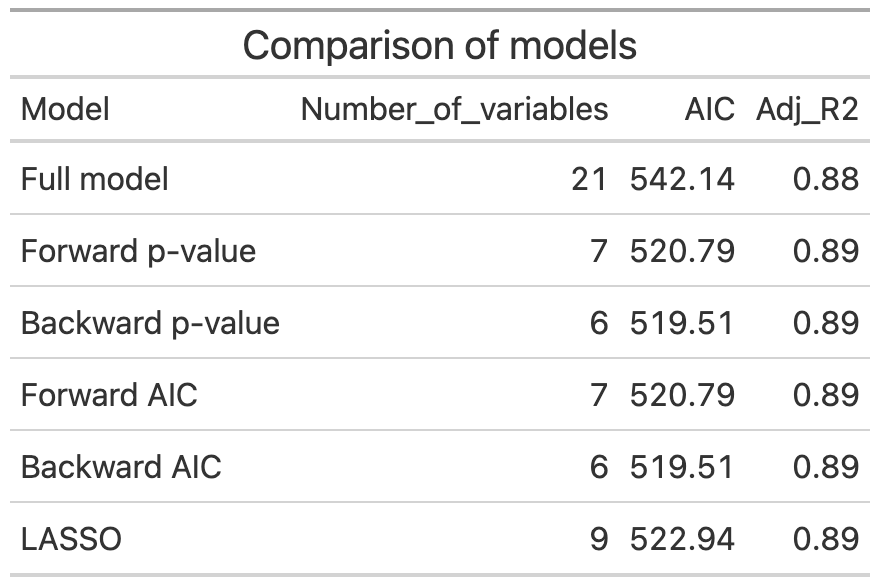
\includegraphics{figures/models/models.png}
	\caption{Comparison of the full model with models resulting of forward/backward selections using p-value and AIC criterion}
	\label{fig:models}
\end{figure}

We compared the full model with forward/backward selections using the p-value criterion and AIC criterion. Each selected model has a slighty better adjusted $R^2$ of $0.89$ compared to the full model with the benefit of being much simpler. Therefore, we choose the model with the less variables. We noticed that the backward elimination select the same variable for the p-value criterion and the AIC criterion. We chose to go for the backward selected model using p-value.

\subsection{Interactions between variables}

We should then try to add interactions betweem variables to our chosen model. We decide to test the following interactions and compare the resulting models with our chosen one,

\begin{itemize}
	\item \textit{infant.deaths} with \textit{measles}
	\item \textit{adult.mortality.high} with \textit{alcohol}
	\item \textit{adult.mortality.very\_high} with \textit{alcohol}
	\item \textit{total.expanditure} with \textit{adult.mortality.low}
	\item \textit{total.expanditure} with \textit{infant.deaths}
\end{itemize}

\begin{figure}[H]
	\centering
	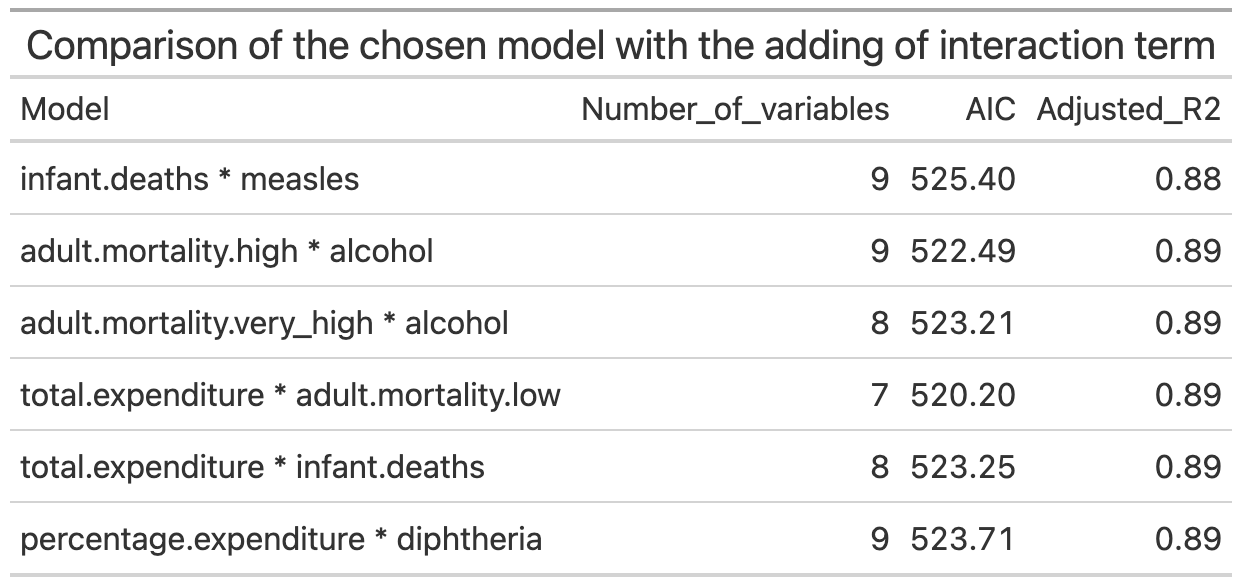
\includegraphics{figures/models/models_interactions.png}
	\caption{Comparison of the chosen model with the adding of an interaction term}
	\label{fig:models_interaction}
\end{figure}

Looking at the adjusted $R^2$, we notice that the different interacting terms do not explain more our target variable (it's even lower for the first interacting term). Moreover, the AIC criterion is worse that the model without any interaction. Therefore, we choose to not add an interaction term.

Our final model is then, 
\begin{align*}
	\textit{life.expectancy} 
		&= \beta_0 + \beta_1 \cdot \textit{total.expanditure} + \beta_2 \cdot \textit{hiv.aids} + \beta_3 \cdot \textit{income.composition.of.resources} \\
		&+ \beta_4 \cdot \textit{adult.mortality.low} + \beta_5 \cdot \textit{adult.mortality.middle} \\
		&+ \beta_6 \cdot \textit{adult.mortality.very\_high}
\end{align*}

\subsection{Verifying underlying hypotheses}

After selecting a model, we want to check the underlying hypothesis of the linear model. We will verify the 3 main hypothesis: homoskedasticity, independance of observations and normality of the residuals. we will also check for outliers, autocorrelation and nonlinearity.

\subsubsection{Nonlinearity}

We can check for nonlinearity by looking at the scatterplot of the residuals ($e_i$) versus the explanatory variables.

\begin{figure}[H]
	\centering
	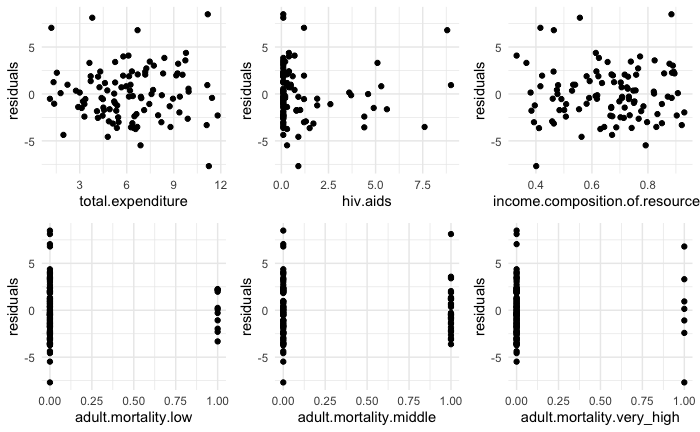
\includegraphics{figures/models/residuals_vs_explanatory.png}
	\caption{scatterplots of residuals versus explanatory variables for the selected model}
	\label{fig:residuals_vs_explanatory}
\end{figure}

We do not see clear nonlinear patterns in the different plots above. Every variable has more or less a linear relation with its residuals. The continuous variable \textit{hiv.aids} has a strange pattern but the nonlinear seems too complicated to infer and would add a lot of complexity to our model. Therefore, we do not take remedial actions.

\subsubsection{Outliers and influential observations}

a) outliers with respect to the explanatory variables

We first try to identify outliers with respect to the explanatory variables $X_{ij}$. They can be identified by studying the leverages that are the diagonal elements of the "hat matrix" $H := X(X^T X)^{-1}X^T$. $X_i$ is an outlier if,
\begin{equation*}
	h_{ii} > \frac{2p}{n} \approx 0.116
\end{equation*}

We find $\textbf{13}$ outliers that are the following rows of our dataset: $6$, $9$, $11$, $23$, $35$, $40$, $49$, $58$, $65$, $82$, $97$, $99$, $100$.

We want then know if the outliers found are influentials for the their fitted values. We use the DFFITS criterion for the i-th observation,
\begin{equation}
	\text{DFFITS}_i = d_i^{\ast} \sqrt{\frac{h_{ii}}{1 - h_{ii}}}
\end{equation}
where $d_i^{\ast}$ are the standardized deleted residuals,
\begin{equation}
	d_i^{\ast} = e_i \sqrt{\frac{n - p - 1}{\text{SSE}(1 - h_{ii}) - e_i^2}} 
\end{equation}

We have a criterion for DFFITS. For $n > 30$, the i-th observation is influential for its fitted value if, 
\begin{equation}
	|\text{DFFITS}_i| > 2 \sqrt{\frac{p}{n}} \approx 0.52
\end{equation}

We find that $\textbf{8}$ observations are influentials for the fitted values: $2$, $9$, $23$, $35$, $49$, $95$, $96$. Therefore, the observations $9$, $23$, $35$, $49$ are outliers and influentials for the fitted values.

\begin{figure}[H]
	\centering
	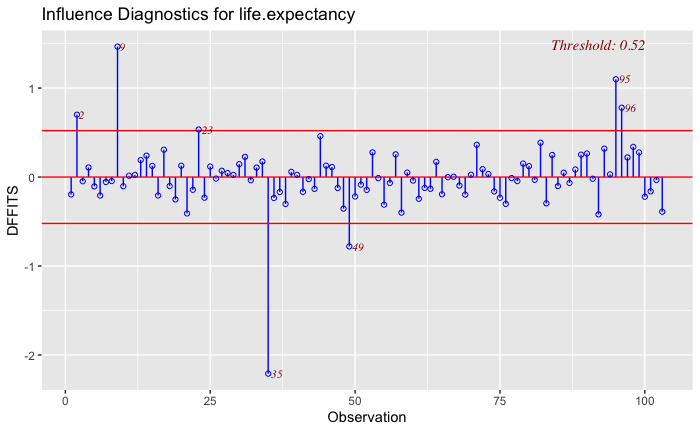
\includegraphics{figures/models/dffits.png}
	\caption{Plot of DFFITS vs observations. Outside the two red lines are the outliers influentials for their fitted values.}
	\label{fig:dffits}
\end{figure}

Now, are they also influentials for the regression coefficients ? We find that the same $\textbf{8}$ observations influentials for the fitted values are also influentials for the regression coefficients. We use the DFBETAS criterion for the i-th observation and k-th coefficient $\hat{\beta}_k$, 
\begin{equation}
	|\text{DFBETAS}_{k,i}| = \frac{\hat{\beta}_k}{\hat{\beta}_{k,i}}{\text{MSE}_i \cdot c_k}, \quad c_k = (X^T X)^{-1}_{kk}
\end{equation}
We have a criterion for DFBETAS. The i-th observation is influential for the k-th coefficient if, 
\begin{equation}
	\text{DFBETAS}_{k,i} > \frac{2}{\sqrt{n}} \approx 0.197
\end{equation}

In the following plots, you can have a look at the differents outliers for each coefficient
\begin{figure}[H]
	\centering
	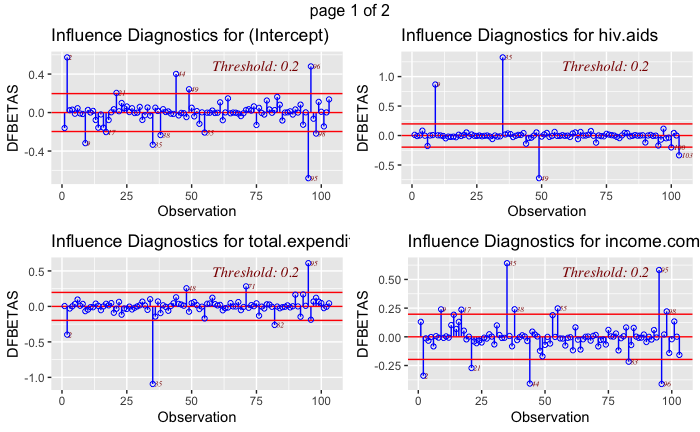
\includegraphics{figures/models/dfbetas_1.png}
	\caption{Plot of DFFITS vs observations. Outside the two red lines are the outliers influentials for the respective variable.}
	\label{fig:dfbetas1}
\end{figure}

\begin{figure}[H]
	\centering
	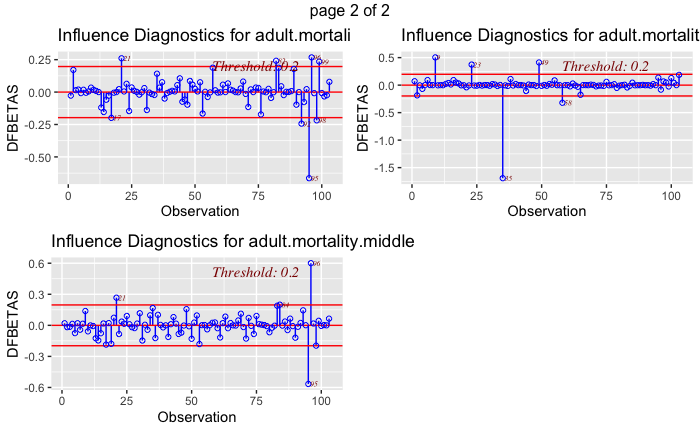
\includegraphics{figures/models/dfbetas_2.png}
	\caption{}
	\label{fig:dfbetas2}
\end{figure}

To summarize this, let's have a look at the Cook's distance $D_i$.

\begin{figure}[H]
	\centering
	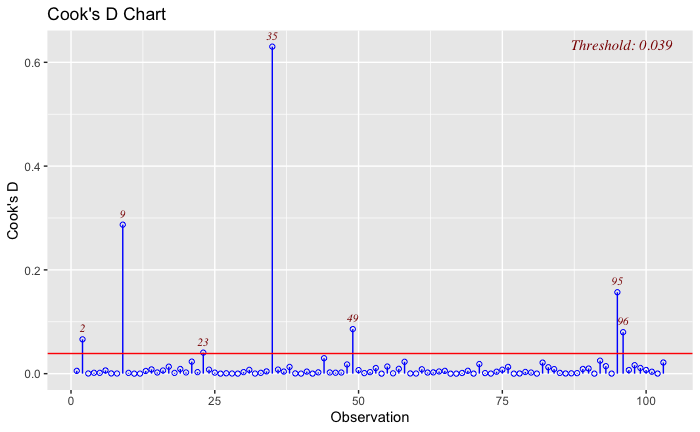
\includegraphics{figures/models/cooks.png}
	\caption{Cook's distance. Outside the red lines are the outliers influentials for the regression coefficients.}
	\label{fig:cooks_distance}
\end{figure}

b) outliers with respect to the response variable

We then identify outliers with respect to the response variable $Y_i$. $Y_i$ is an outliers if $d_i^{\ast} > t_{n-p-1;1 - \frac{\alpha}{2}}$. For a level of significance of $\alpha = 0.05$, we have $t_{94 ; 0.975}$ and we find that the observations $2$, $9$, $95$ and $96$ are outliers for the response variable.

\subsubsection{Multicollinearity}

We verify now if we have any multicollinearity problem. We saw in the descriptive statistic section that some variables were highly correlated. These high pairwise correlations could lead to multicollinearity problem but it is not always the case.

Let the full model be, 
\begin{equation}
	Y = X\beta + \varepsilon
\end{equation}

To check for multicollinearity, we can use the \textbf{Variance inflation factor (VIF)} that is defined by for the coefficient $\hat{\beta}_k$,

\begin{equation}
	\text{VIF}_k = \frac{1}{1 - R^2_k}, \quad k = 1,...p-1
\end{equation}

where $R^2_k$ is the coefficient of determination of a regression of $X_k$ on $X_1,\dots,X_{k-1},X_{k+1},\dots,X_{p-1}$. Multicollinearity leads to an "ill-conditionned" matrix $X$. As a consequence, this matrix is numerically instable and becomes difficult to invert. Therefore, the OLS estimator $\hat{\beta}$ cannot be "correctly" computed.
We have multicollinearity problem if the \textbf{VIF} is greater than $10$ and if the \textbf{average VIF} is much greater than $1$. We can also check the tolerance which is $1 - R^2_k$.

% In the appendix (\ref{fig:vif_full_model}), you can find a table with the VIF and tolerance for each variable of the full model. We notice a multicollinearity problem for the variables \textit{gpd} (with VIF $= 13.10$) and \textit{income.composition.of.resources} (with VIF $= 12.72$). These two have tolerance of $0.08$. Furthermore, the average VIF is $4.67$. %Therefore we can already remove these two variables from our model.

% In order to fix this multicollinearity problem, we can perform a \textbf{Ridge regression} that is similar to the OLS in the sense it minimizes the SSR but it also adds a constraint on the $L_2$ norm (euclidean) for $\beta$. The constraint is,
% \begin{equation}
% 	||\beta||^2_2 \leq t
% \end{equation}
% where $t \in \R$ is a parameter to be determined.

\begin{figure}[H]
	\centering
	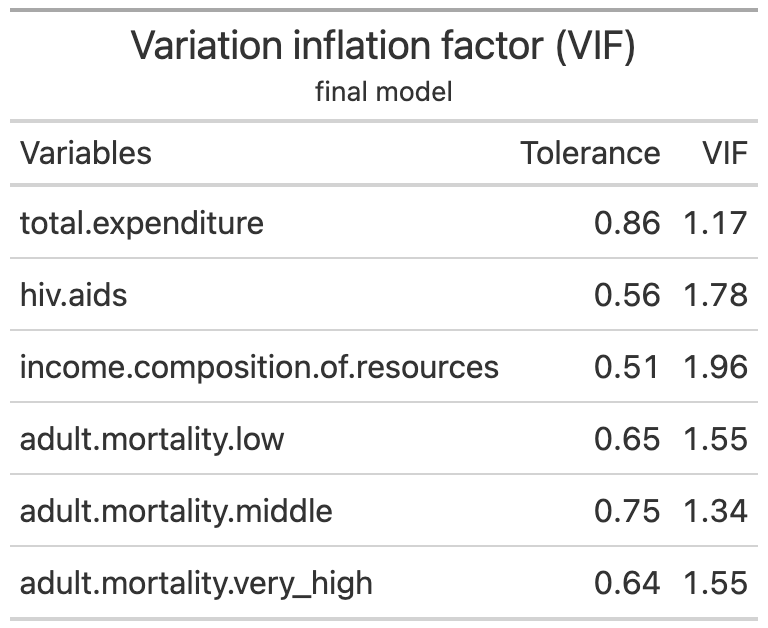
\includegraphics{figures/models/vif_final_model.png}
	\caption{VIF for the selected model}
	\label{fig:vif_final_model}
\end{figure}

We notice we do not have any variable with a \textbf{VIF} > 10 so we do not have multicollinearity problem.

\subsubsection{Heteroskedasticity}

We can try to check for heteroskedasticity by looking at the plot of the residuals versus the fitted response variable.

\begin{figure}[H]
	\centering
	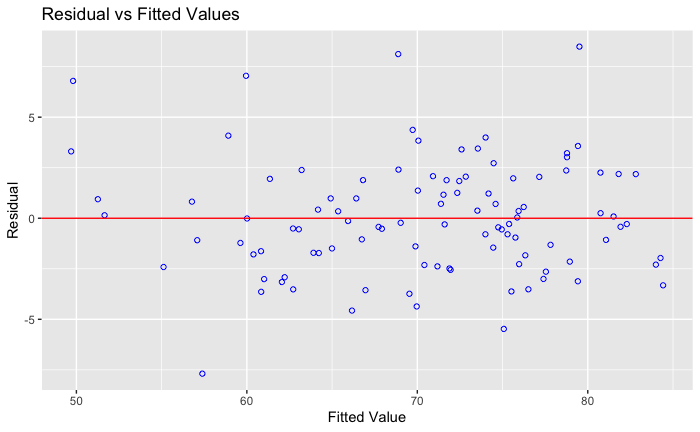
\includegraphics{figures/models/residuals_vs_fitted_response.png}
	\caption{scatterplots of residuals versus fitted response variable}
	\label{fig:residuals_vs_fitted_response}
\end{figure}


However, it's not that clear with plot if there is heterosckedasticity problem or not. The best way to determinate if there is heteroskedasticity is to perform the \textbf{White test}. The hypothesis are,
\begin{align*}
	H_0&: \text{there is homoscedasticity} \\
	H_1&: \text{there is heteroskedasticity}
\end{align*}

The result is,
\begin{figure}[H]
	\centering
	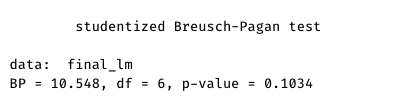
\includegraphics{figures/models/white_test.png}
	\caption{Result of White test for homoeskedastiscity}
	\label{fig:white_test}
\end{figure}

The p-value of the \textbf{White test} is $0.01729$. At a significance level of $\alpha = 0.05$, we reject the null hypothesis and therefore we can conclude there is \textbf{heterosckedasticity}.

% TODO: taking remedial actions

% box-cox does not resolve heterosckedastiscity
We tried to make a Box-Cox transformation of the dependant variable but unfortunately, this did not fix the heterosckedasticity.

\subsubsection{Autocorrelation}

We can check for autocorrelation by performing the \textbf{Breusch-Godfrey test}. The hypotheses are,
\begin{align*}
	H_0&: \text{there is no autocorrelation} \\
	H_1&: \text{there is autocorrelation}
\end{align*}

% TODO: show output of the Breusch-Godfrey test
\begin{figure}[H]
	\centering
	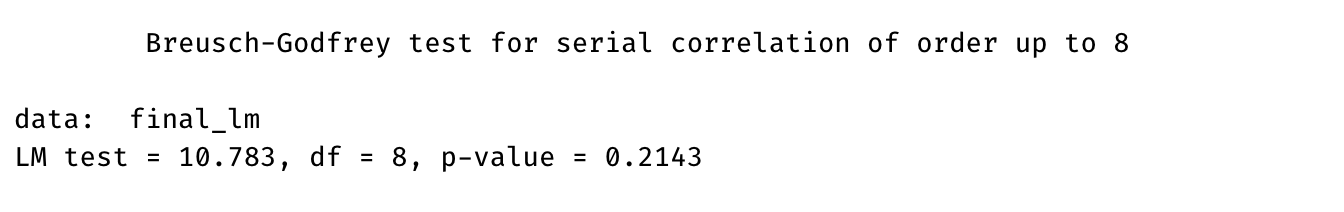
\includegraphics{figures/models/Breusch-Godfrey_test.png}
	\caption{Result of Breusch-Godfrey test for autocorrelation}
	\label{fig:breusch-godfrey-test}
\end{figure}

The p-value of the \textbf{Breusch-Godfrey test} is $0.2143$. At a significance level of $\alpha = 0.05$, we fail to reject the null hypothesis and therefore we can conclude there is \textbf{no autocorrelation}. 

\subsection{Normality of the residuals}

Considering the Normal Q-Q plot of the residuals comparing the quantiles of the residuals versus the quantiles of a normal distribution. If the residuals are normal, the points on the following plot should follow the straight line,

\begin{figure}[H]
	\centering
	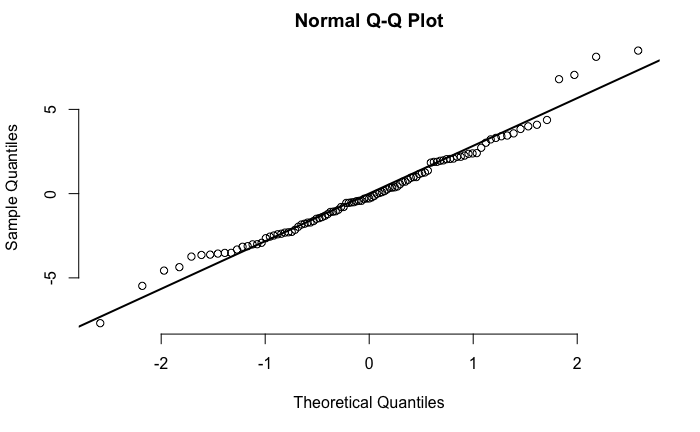
\includegraphics{figures/models/normal-qq-plot.png}
	\caption{Normal QQ-plot}
	\label{fig:normal-qq-plot}
\end{figure}

Looking at this plot, we see that globally the points follow the straight line so the residuals are normals.  

To ensure there is no a problem of normality for the residuals, we can perform a \textbf{Jarque Bera test}. 

Let $S$ be the skewness and $\kappa$ of the residuals. The \textbf{Jarque Bera test} is given by, 
\begin{equation}
	\text{JB} = \frac{n}{6} \left(S^2 + \frac{(\kappa - 3)^2}{4} \right)
\end{equation}

The hypothesis are, 
\begin{align*}
	H_0&: \text{JB} \sim X^2_2 \\
	H_1&: \text{residuals are not normally distributed}
\end{align*}

\begin{figure}[H]
	\centering
	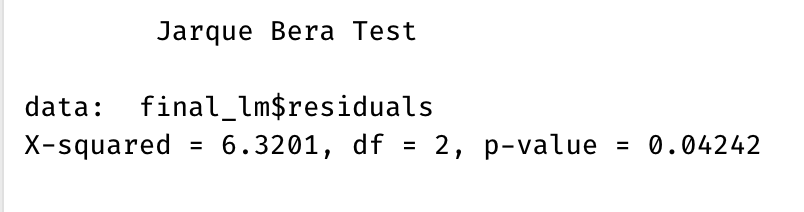
\includegraphics{figures/models/jarque-bera_test.png}
	\caption{Result of Jarque-Bera test}
	\label{fig:jarque-bera-test}
\end{figure}

The p-value of the \textbf{Jarque Bera test} is $0.042$. At a significance level of $\alpha = 0.05$, we fail to reject the null hypothesis and therefore we can conclude the \textbf{residuals are normaly distributed}. 

\section{Significance of estimated coefficients}

We perform t-tests of estimated coefficients in order to test their significance. For t-tests, we use the following null and alternative hypotheses for each regression coefficient: 
\begin{align*}
	H_0&: \beta_i = 0 \\
	H_1&: \beta_i \neq 0
\end{align*}

\begin{figure}[H]
	\centering
	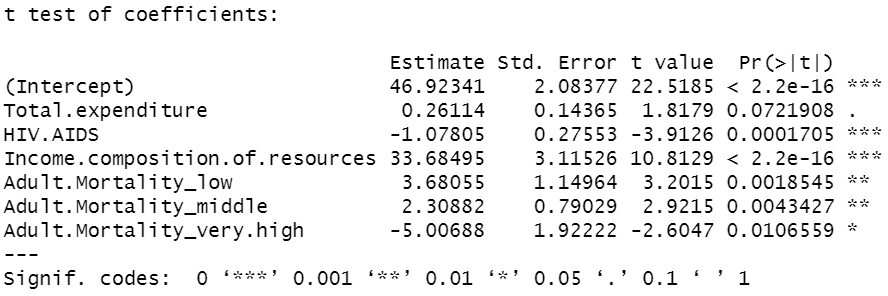
\includegraphics{images/test_t_coefficients_robust_inference.PNG}
	\caption{Output of t-test of coefficients}
\end{figure}

On the basis of the p-values, we can reject the null hypothesis for all the coefficients. We can conclude that all the coefficients are statistically significant at a level of significance of 10\%. At a significance level of 5\%, the “adult mortality very high” coefficient is no longer statistically significant. \\

On the basis of the estimates, we can say that the effect of low and middle adult mortality rates on life expectancy are positive while the effect of a very high adult mortality rate on life expectancy is negative and stronger. From the regression output, we see that the estimate of the regression coefficient for “Adult mortality very high” is -5.007. This signifies that on average, a country with a very high adult mortality rate has a life expectancy of 5 years less. On the contrary, a country with a low  adult mortality rate has a life expectancy higher of 3 years on average and 2 years for a country with a moderate adult mortality rate. 

\section{Linear combination  of coefficients}

 We want to test the hypothesis that there exists a linear combination between two regression coefficients: \begin{equation*}
     \beta_4 = \beta_5
 \end{equation*} 
 With this, we want to test if these two coefficients are equal. We can also write it as follow: \begin{equation*}
     \beta_4 - \beta_5 = 0
 \end{equation*}
We formulate the null and alternative hypotheses : 
\begin{align*}
	H_0&: \beta_4 - \beta_5 = 0 \\
	H_1&: \beta_4 - \beta_5 \neq 0
\end{align*}

\begin{figure}[H]
	\centering
	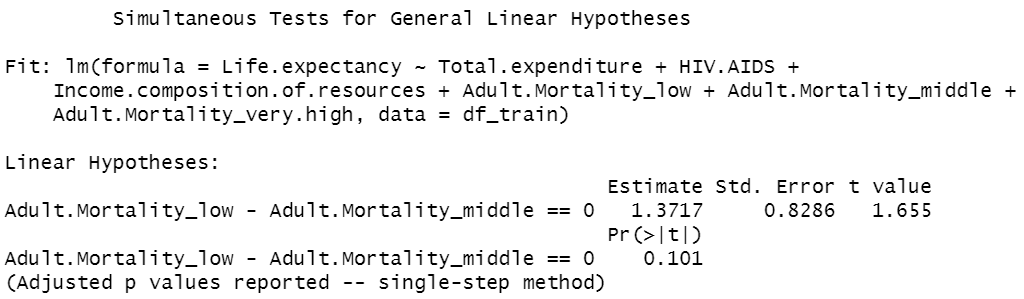
\includegraphics{images/linear_combination_of_coeff.PNG}
	\caption{Output of linear combination test}
\end{figure}

Since the p-value (0.101) is larger than the significance level of 0.05, we fail to reject the null hypothesis that these two regression coefficients are equal. This signifies that a country with a low adult mortality rate and a country with a moderate adult mortality rate could have the same reduction in years of life expectancy if all the other effects remain constant. 

\section{Coefficients equal to zero}

We test a subset of coefficients equal to zero. In this case, we test the coefficients corresponding to all qualitative variables equal to zero. Hence, the null and alternative hypotheses are the following :

\begin{align*}
	H_0&: \beta_4 = \beta_5 = \beta_6 = 0 \\
	H_1&: \text{at least one of these is not equal to zero}
\end{align*}

\begin{figure}[H]
	\centering
	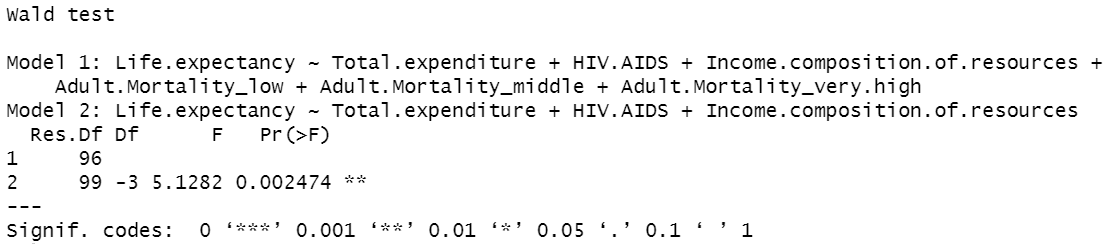
\includegraphics{images/wald_test_subset_coeff_zero.PNG}
	\caption{Output of Wald test}
\end{figure}

The p-value is 0.0025 which is below the significance level of 0.05. We can thus reject the null hypothesis. We can conclude that there is sufficient statistical evidence that the different categorial variables corresponding to adult mortality rates explain life expectancy. 

\section{Prediction interval}

We calculate a 95\% prediction interval for the 26 observations excluded from the dataset in the beginning. We conclude that almost all the intervals cover the excluded observations. The last observation of the test dataset is the only one not covered by the corresponding 95\% prediction interval. However, if we take the 99\% prediction interval, this observation is contained in the prediction interval.
